\scanpage{15}
\uline{Exercise}\qquad Regular realization of a polygon.

Let $\deleted{V}E$ be a Euclidean affine plane over $\mathbb{R}$ (with positive definite metric on \unsure{the space|the space|the space} $V$ of translations). A rectilinear realization of a polygon $(S,A,R)$ is said to be \uline{regular} if all the sides of the polygon have $=$
% The two-line addition stands to the right of longueur. Its enclosing line is
% open at the left-hand tail; the separate comma remains beside that opening.
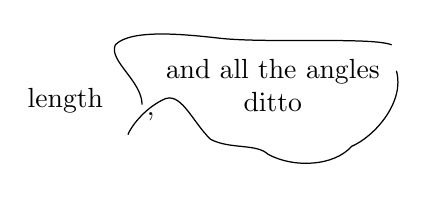
\begin{tikzpicture}[baseline=(longueur.base),x=1cm,y=1cm]
  \node[anchor=base west,inner sep=0pt] (longueur) at (0,0) {length};
  \node[anchor=base,inner sep=0pt] at (1.57,-.10) {,};
  \node[anchor=center,inner sep=0pt] at (3.12,.29)
    {\inserted{\shortstack{and all the angles\\ditto}}};
  \draw[line width=.45pt]
    (1.46,.04) .. controls (1.46,.34) and (1.03,.60) .. (1.12,.80)
    .. controls (1.32,1.01) and (2.04,.93) .. (2.48,.88)
    .. controls (3.12,.82) and (4.38,.90) .. (4.63,.80);
  \draw[line width=.45pt]
    (4.69,.47) .. controls (4.80,.08) and (4.42,-.36) .. (4.12,-.49)
    .. controls (3.90,-.74) and (3.39,-.77) .. (3.06,-.59)
    .. controls (2.91,-.45) and (2.58,-.53) .. (2.33,-.40)
    .. controls (2.09,-.17) and (1.95,.23) .. (1.72,.10)
    .. controls (1.48,-.02) and (1.32,-.24) .. (1.28,-.34);
\end{tikzpicture}
\uline{regular} \deleted{and} \uline{\unsure{normalized|normalized}} if the said length is $1$.

a) Existence, thanks to cyclotomic equation $z^n=1$ in $\mathbb{C}$.

b) Prove that if $(V\deleted{\unsure{,}}\supset P\deleted{\unsure{,}}\supset\deleted{\unsure{A|B}}S)$ and $(V'\supset P'\supset S')$ are two $n$-polygons ($n\geq3$) equipped with a \uline{regular} rectilinear \unsure{realization|realization} (resp \unsure{normalized|normalized}) there exists a \deleted{\unsure{isometry|isometry}} similarity (resp \unsure{isometry}) \deleted{\uline{unique}} from $V$ onto $V'$, which transforms $P$ and $P^{\unsure{\prime|!}}$, $S$ into $S'$; \tikz[baseline=(cancel.base),x=1em,y=1em]{
  \node[inner sep=0pt,anchor=base west] (cancel) at (0,0) {\deleted{if $V\unsure{;|,}P,S$}};
  % The cancellation has a separate hooked return at its left end.
  \draw[line width=.4pt] (-.55,.25) .. controls (-.35,-.02) and (.12,-.06) .. (.62,.3);
  \draw[line width=.4pt] (-.55,.25) -- (-.12,.35);
} more precisely, for every isomorphism (combinatorial) from $(\deleted{P}\unsure{S},A,R)$ onto $(S',A',R')$, $\exists\,\unsure{\vert|1}$ similarity
% The addition is above de V. A rising curved arrow runs beneath it and ends
% just above the corrected V; the baseline text remains de V sur V'.
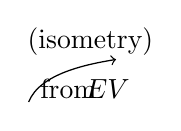
\begin{tikzpicture}[baseline=(de.base),x=1cm,y=1cm]
  \node[anchor=base west,inner sep=0pt] (de) at (.16,0) {from};
  \node[anchor=base,inner sep=0pt] (oldV) at (1.02,0) {$\deleted{\unsure{E}}V$};
  \node[anchor=base west,inner sep=0pt] at (0,.63) {\inserted{(isometry)}};
  \draw[->,line width=.45pt] (.02,-.05)
    .. controls (.16,.31) and (.76,.43) .. (1.13,.49);
\end{tikzpicture}
onto $V'$ which induces it. \deleted{Show that}

\deleted{\unsure{Ex|Corollary}}\quad\uline{Corollary} Notion of affine hull (or linear, thanks to: center of
% The addition is above gravité), with its independent closing parenthesis.
% The curved lead meets short forked strokes and a longer oblique stroke.
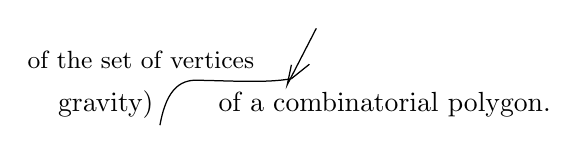
\begin{tikzpicture}[baseline=(gravite.base),x=1em,y=1em]
  \node[anchor=base west,inner sep=0pt] (gravite) at (0,0) {gravity)};
  \node[anchor=base west,inner sep=0pt,font=\small] at (-1.1,1.55)
    {\inserted{of the set of vertices}};
  \node[anchor=base west,inner sep=0pt] at (5.8,0) {of a combinatorial polygon.};
  \draw[line width=.45pt] (3.7,-.5)
    .. controls (3.95,.9) and (4.5,1.18) .. (5.2,1.12)
    .. controls (6.3,1.1) and (7.6,1.02) .. (8.45,1.18);
  \draw[line width=.45pt] (8.45,1.18) -- (9.1,1.70);
  \draw[line width=.45pt] (9.35,3.0) -- (8.30,.96) -- (8.45,1.68);
\end{tikzpicture}

\deleted{\unsure{If|Let}} Orientation of the polygon $\longleftrightarrow$ orientation of its hull
% Two detached dark points below the right end of the last line: writing versus surface trace remains uncertain.
\par\vspace{2.5\baselineskip}\noindent\hfill
\unsure{\tikz[baseline=-.3ex]{
  \fill (0,0) ellipse (.055em and .035em);
  \fill (.14em,.24em) ellipse (.035em and .055em);
}}\hspace*{2em}\par
% archive sheet number: 14
